\section{IoT as a Socio-technical System}
\label{sec:IoT_socio-techical}
Since 1999, when Ashton \cite{ashton2011internet} coined the term \textbf{Internet of Things (IoT)}, while he was introducing RFID technology in the context of supply-chain management, the meaning of the term has evolved. Today, International Telecommunication Union (lTU) defines IoT as the worldwide network of interconnected objects uniquely addressable based on standard communication protocols. Such a definition focuses only on the technical side of IoT. From the technical aspect, the IoT can be divided into three following layers:
\begin{itemize}
	\item comprehensive sensing (perception layer),
	\item reliable transmission (network layer), and
	\item intelligent processing (application layer).
\end{itemize}
Nevertheless, the envisioned IoT represents a socio-technical, instead of only technical system, as the interconnected objects are intended to interact also with people and society \cite{atzori2014smart}. However, as discussed in Introduction for socio-technical systems in general, it is also the case for IoT that the focus among engineers and computer scientists was mainly on the technical side. Interestingly, even some of the ideas for the \textit{Social IoT (SIoT)} \cite{atzori2012social,guinard2010sharing,atzori2014smart} discuss the convergence of social networks with IoT mainly with the intention to optimize the interactions among the IoT objects. There is sometimes very little attention in such studies on the interrelationship of IoT with the human psychological and social aspects \cite{atzori2012social,guinard2010sharing}. 

The discussion on IoT should also tackle on another term that is often used interchangeably with IoT -- \textbf{ubiquitous computing} coined by Weiser \cite{weiser1991computer}. Ubiquitous computing is defined as ``the physical world that is richly and invisibly interwoven with sensors, actuators, displays, and computational elements, embedded seamlessly in the everyday objects of our lives, and connected through a continuous network'' (ibid.). In other words, while the Internet has led to the interconnection of people at an unprecedented scale, the IoT is expected to interconnect also the objects around us, leading to a smart environment \cite{gubbi2013internet}. %We see that researches talking about IoT mainly describe connected devices, while ubiquitous computing focuses on the smart environment in which computing is pervasive. 
%Hence, the two terms take a different stance and focus on different aspects of what is envisioned to become the \textit{Future Internet}. 
The IoT vision put forward by Weiser \cite{weiser1991computer} led to a fruitful new field within computer science (ubiquitous computing). However, 15 years later, Rogers \cite{rogers2006moving} offered a constructive critique of this vision. Namely, Rogers argued that we should move from a \textit{computing approach} (technical aspects) to a \textit{human approach} (social aspects) in developing the smart environment. In particular, the original vision suggested that ubiquitous computing can lead to an environment that is predicting and adapting to the people's needs, while the people were considered passive elements (i.e., technological determinism). Rogers argues the opposite: ``To make this happen, however, requires moving from a mindset that wants to make the environment smart and proactive to one that enables people, themselves, to be smarter and proactive in their everyday and working practices.''

The effects of critique, such as the one by Rogers, are seen in researches increasingly adopting the human and social approaches in discussing the IoT \cite{ning2011future,guo2012opportunistic,tomasini2017effect}. One human-centric vision is illustrated by the \textit{Opportunistic IoT} \cite{guo2012opportunistic,guo2013opportunistic}. The authors explain that the IoT should be designed with the bidirectional effects between people and loT in mind. As presented in Fig.\ \ref{fig:opportunisticIoT}, in addition to object-object interaction, the IoT design should also consider human-object, human-environment and human-human interactions. Moreover, it is also recognized that the IoT design needs to consider different aspects of human behaviour, such as mobility \cite{tomasini2017effect}, preferences \cite{kowshalya2016community}, and homophily \cite{atzori2012social}. In the light of such ideas, Ortiz et al.\ \cite{ortiz2014cluster} revisit previously introduced ideas of {SIoT} (that still treat IoT only as technical system) and provide a more comprehensive vision of it -- one that treats the IoT as a socio-technical system.

\begin{figure}
	\sidecaption
	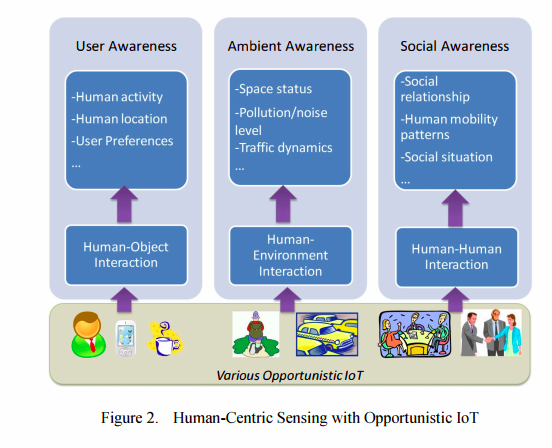
\includegraphics[scale=.55]{img/opprtunisticIoT}
	\caption{Human-centric Opportunistic IoT \cite{guo2012opportunistic}}
	\label{fig:opportunisticIoT} 
\end{figure}



\subsection{IoT for the Smart Grid}
\label{sec:IoTSG}
Yun and Yuxin \cite{yun2010research} discuss the possibilities of the IoT to bring about the \textit{smart grid} through sensors, novel telecommunications and computing technologies. The sensors, such as smart, temperature, and illumination meters, collect energy and environmental data. They can also form a high-speed, real-time and bidirectional connection between the consumers, utilities and the electrical grid. It is envisioned that such an improved data collection and communication can support the decision making and in turn improve the overall efficiency of the grid. Interestingly, the technology at the heart of the IoT, the Internet itself, consumes up to 5\% of the total energy spent today in the world. Given the expectation of connecting billions of new devices, this consumption is expected to go up \cite{gubbi2013internet}.	

One of the key application areas of IoT is envisioned to be in the smart residential buildings \cite{schatten2014smart}. Among a number of smart devices that are interconnected and installed in such buildings, the devices that support the smart grid development, such as smart energy, temperature, illumination and other types of environmental meters,  will also be present. According to Zygiaris' Smart City Reference Model \cite{zygiaris2013smart}, there are different innovation layers that can be used to describe the smart innovation and development characteristics within the smart cities. IoT should play an important role in several of those layers: from the interconnection layer with a number of sensors and actuators, through the integration layer monitoring those smart devices, to the intelligent applications layer making use of the real-time data. In China, in particular, among the largest portions of the IoT market is envisioned for the development of the smart grid \cite{shin2014socio}.

When it comes to the smart grid, there are the dimensions of demand and supply of energy that can be tackled. Tackling the demand should involve the users \cite{verbong2013smart}. While the focus on technology is still too strong and some smart grid players still perceive the users themselves as the barriers to the smart grid development process, we instead need to understand to what extent the users can act as solution to the sustainability pathway. IoT is predicted to enable transparent energy consumption information of different services in cities, from lighting, through public transport, to heating and air conditioning of public spaces \cite{zanella2014internet}. Moreover, the real-time, bidirectional connectivity between the utilities, grid and the users is suggested to lead to the improved overall efficiency of the grid \cite{yun2010research,li2011applications}. Finally, in the future smart homes, devices are expected to cooperate, actively share their energy and participate in building wide energy management systems \cite{karnouskos2010cooperative}. It is apparent how in such a context, where IoT meets the smart grid, innovative services and business applications emerge, but also security, privacy and trust gain novel importance.

\begin{svgraybox}
Through this chapter, we review the literature on applying IoT to support the design and development of the smart grid.
\end{svgraybox}
